\documentclass[final]{ukthesis}
%you must include these 2 packages.
\usepackage[pdfauthor={Jack Bandy},
            pdftitle={The Title},
            pdfsubject={The Subject},
            pdfkeywords={Some Keywords},
            pdfproducer={Latex with hyperref},
            pdfcreator={latex->dvips->ps2pdf},
            pdfpagemode=UseOutlines,
            bookmarksopen=true,
            letterpaper,
            bookmarksnumbered=true]{hyperref}
\usepackage{memhfixc}
\usepackage{graphicx}
\graphicspath{{./figures/}}
%%%%%%%%%%%%%%%%%%%%%%%%%%%%%%%%%%%%%%%%%%%%%%%%
\begin{document}
%author data
\author{Jack Bandy}
\title{INTERACTIVE MACHINE LEARNING FOR WORD RECOGNITION ON DAMAGED HANDWRITTEN DOCUMENTS}
\abstract{an abstract}
\advisor{Brent Seales}
\keywords{keywords go here}
\dgs{Miroslaw Truszczynski}
%the title pages
\frontmatter
\maketitle
\begin{acknowledgments}
Acknowledge people/things here
\end{acknowledgments}
\tableofcontents\clearpage
\listoffigures\clearpage
\listoftables\clearpage
%----------------------------------------------
\mainmatter


%%
%
%
% Introduction Chapter
%
%%
\chapter{Introduction}


%
% Related Work
%
\section{Related Work}
For several decades, researchers have been developing methods for automated character and word recognition. These methods take some photograph(s) of printed or handwritten text as input, and produce a transcript of that text as output. This section provides a brief summary of methods which have influenced the course of this research area, including advances in handwriting recognition, printed text recognition, and handwritten word spotting.

The nomenclature for these related tasks can be somewhat inconsistent in the literature. For the purposes of this paper, ``handwriting recognition'' differs from ``handwritten word spotting'' in that the former aims to create full transcriptions while the latter merely locates and/or recognizes instances of a given word within a document. ``Printed text recognition,'' although it uses many of the same methods, refers to projects that examine machine-printed texts. The consistency of character representations and thus word representations drastically changes the task, so a distinction is necessary.

% Text Recognition Subsection
\subsection{Text Recognition}
``Text recognition'' here refers to recognizing {\em printed} texts, not handwritten texts. From a technical standpoint, automatic text recognition is the task of turning an image into the text within the image.

Object character recognition (OCR) on scans of printed documents has seen success since as early as the 1980s \cite{mantas1986overview,govindan1990character}. Due to the consistency of letter shapes and sizes, fairly simple techniques for pattern recognition could accurately classify characters in the same font family. However, as early as 1987, font and size constraints were no longer needed. The authors of \cite{kahan1987recognition} demonstrated a system that accurately classified mixtures of dissimilar fonts of varied sizes.

Gradually, more and more constraints were eliminated. After \cite{kahan1987recognition} removed the need for font and size assumptions, the race was on to eliminate constraints such as alignment, color, contrast, and more. Eventually, the task of printed text recognition was one that could be done ``in the wild,'' \cite{smith2007overview,wang2012end,jaderberg2016reading} with essentially no assumptions about the nature of the text. Especially important for ``in the wild'' recognition was eliminating the segmentation step, as in \cite{rusinol2015efficient}, such that regions of text could be found without a processing phase devoted to localization. The ideal system, then, would be able to recognize text in any image in which a human could see text.

An important benchmark dataset for this kind of text recognition is Street View Text (SVT) \cite{wang2010word}. SVT was harvested using pictures from Google Street View, and thus contains a heterogeneous collection of word images with a variety of fonts, colors, backgrounds, and more. (Despite the variations, word images in this set do not include handwritten characters.) The SVT dataset was released in 2010, and by 2012, \cite{wang2012end} demonstrated state-of-the-art performance for both character recognition and word recognition by training on images from the dataset. The high degree of accuracy was achieved via unsupervised feature learning and convolutional neural networks.

Even before 2012, many researchers realized that convolutions provide an ideal mechanism for recognizing the shapes of different letters. Others have taken more general approaches to text recognition via CNNs \cite{wang2012end,jaderberg2016reading}, . The network architectures from these papers are, on the whole, restrictively large, whereas both architectures from my experiments were able to run on my laptop.


% Handwriting Recognition Subsection
\subsection{Handwriting Recognition}
Although modern methods for printed text recognition overlap methods for handwriting recognition, especially with CNNs for ``in-the-wild" recognition, the convergence happened after years of parallel research. Handwriting recognition can be divided into two major categories, ``online" handwriting recognition and ``offline" handwriting recognition. In the former, software tracks the location of a writing utensil as a user moves it across some surface to produce letters and words, and the precise location and motion of the utensil helps reveal the intended writing. For example, UNIPEN \cite{guyon1994unipen}, a benchmark dataset for online handwriting recognition, includes ``pen trajectory" data that specifies when and where the pen touched down and lifted up, as well as the coordinates for the path of the pen.

More relevant to this project is the task of offline handwriting recognition, in which the input comprises only a picture of the handwriting and no additional information about its creation. A canonical example of the text recognition task is the MNIST dataset \cite{lecun1998mnist}. MNIST comprises grayscale images of individual handwritten digits, 0 to 9, and the objective is to classify each image into the digit written inside of it. Machine learning researchers have been using this task as a benchmark for several decades \cite{bottou1994comparison}, with error rates well below 1\% since 2003 \cite{kussul2004improved}.

Projects using MNIST and similar datasets are premised upon many constraints. For example, a very small vocabulary or character set could be recognized if they were properly aligned and segmented, but as soon as a text ventured outside those constraints (variations on letters, misspelled words, new characters, etc.), the system would falter. Even moderately successful recognition on unconstrained datasets did not exist until the early 2000s.

This changed with the use of hidden Markov Models (HMMs) \cite{marti2001using,bunke2004offline,el1999hmm}. With statistical models built for specific languages, character and word recognition accuracies improved to over 85\% (varying with respect to the test corpus). More impressively, these results came on { \em unconstrained} texts.

While HMMs made the way for unconstrained datasets, many demonstrations were still using the IAM dataset \cite{marti2002iam}, an ad-hoc database for researchers. In other words, {\em truly} unrestricted handwriting recognition was still a long way off even after the strides made by HMMs. Moving forward, a collection of George Washington letters became the de-facto standard. This dataset comprised hundreds of manuscript pages from the Library of Congress, handwritten by George Washington's secretaries.

In the mid-2000s, even state-of-the-art HMM methods yielded word error rates around 50\% on datasets such as the George Washington collection. But around this time, researchers began taking a new angle at the problem. Specifically, projects focused on the process of ``handwriting retrieval,'' rather than attempting complete transcriptions. Such projects allow users to query a dataset of images for a given word, and essentially scans the images for visual matches of that word. For example, \cite{rath2004search} presents a word retrieval system that achieves 63\% mean average precision scores on the George Washington collection.

In \cite{rath2007word}, this approach is formalized as a viable way to generate a searchable index of handwritten papers. Their method of ``wordspotting'' turns the search problem into a clustering problem, where word images that are ``closest'' to the query word are considered matches. Wordspotting is considered more thoroughly in the following section, however it is crucial to note that this approach eliminated the need for recognizing words before retrieval. In other words, matching is done in real-time.

Building upon the success of wordspotting techniques and HMMs, \cite{howe2009finding} takes a step further and first detects {\em characters} in a word, before inferring a word using an ensemble of HMMs. This approach allowed the recognition of words that were never seen during training, and established new standards for the George Washington dataset.

By the time ensemble HMMs came onto the scene, neural networks were already penetrating the field of handwriting recognition \cite{fernandez2007application}. By 2010, advanced techniques such as bidirectional long short-term memory (BLSTM) were successfully applied to wordspotting \cite{wang2010word} and outperformed other methods. Finally, recurrent neural networks \cite{frinken2012novel} eliminated the need for word segmentation in addition to improving state-of-the-art performance on recognition tasks.

More recently, convolutional neural networks (CNNs) have become the state-of-the-art approach for text recognition on handwritten documents \cite{zhong2016spottingnet,sudholt2016phocnet}. Many of these approaches overlap text recognition methods mentioned in the previous section, and in fact, recent neural networks are designed to recognize both printed text and handwritten text.

% Highly relavant stuff
\subsection{Word Spotting on Damaged Handwritten Documents}
In this section, the scope of related projects is narrowed down from all handwriting recognition systems, and I examine research related to word spotting on historical documents.

As previously mentioned, \cite{rath2007word} formalized the idea of wordspotting. However, the concept was originally proposed in \cite{manmatha1996word}, which clustered similar words to be annotated by users, and reported success for documents written by a single person in high-quality handwriting.




%
% Motivation
%
\section{Motivation}
On the surface, optical character recognition, word recognition, and handwriting recognition appear to be solved problems. As detailed in the previous section, the explosion of machine learning research in recent years has led to drastic improvements in performance on these tasks, and many advancements have even found their way to consumer products. For example, everyday software allows users to search within scans or photographs of printed typeface, and note-taking software can now interpret penmanship that would be indecipherable to many human readers.

However, the process of transcribing ancient documents presents a niche area of text recognition which is not addressed well by standard approaches. Many historical documents, including those reviewed in this project, were meticulously transcribed with legibility comparable to typeface, suggesting that automated transcription would be straightforward. But over time, these documents have incurred damage of all different kinds. The characters originally may have looked like typeface, but after hundreds of years of human handling, physical corrosion, chemical decay, and other processes, reading certain parts of these documents is an arduous task even for skilled textual analysts. For such cases, neither fully human transcription nor fully automated transcription is ideal.

While fully manual transcription is the most accurate solution, it is incredibly time-consuming for larger documents. Moreover, on damaged documents, skilled papyrologists are required to decipher texts. In short, human transcription is often prohibitively costly in terms of time and skilled personnel.

A fully automated transcription algorithm may successfully transcribe certain portions of a historical document, but the damaged portions can distort the algorithm's output to the point of being unusable. This is especially true in cases where letters are literally missing. This is especially true for OCR algorithms which assume constant width, spacing, and more within a document.

An ideal solution would leverage automated transcription for the undamaged portions, and allow a human reader to fill in any gaps. A framework for this hybrid approach is presented in \cite{schaekermann2016resolvable}, which also provides an elegant schematic of the approach in Figure \ref{fig:hcml-schematic}.


\begin{figure}[t]
\begin{center}
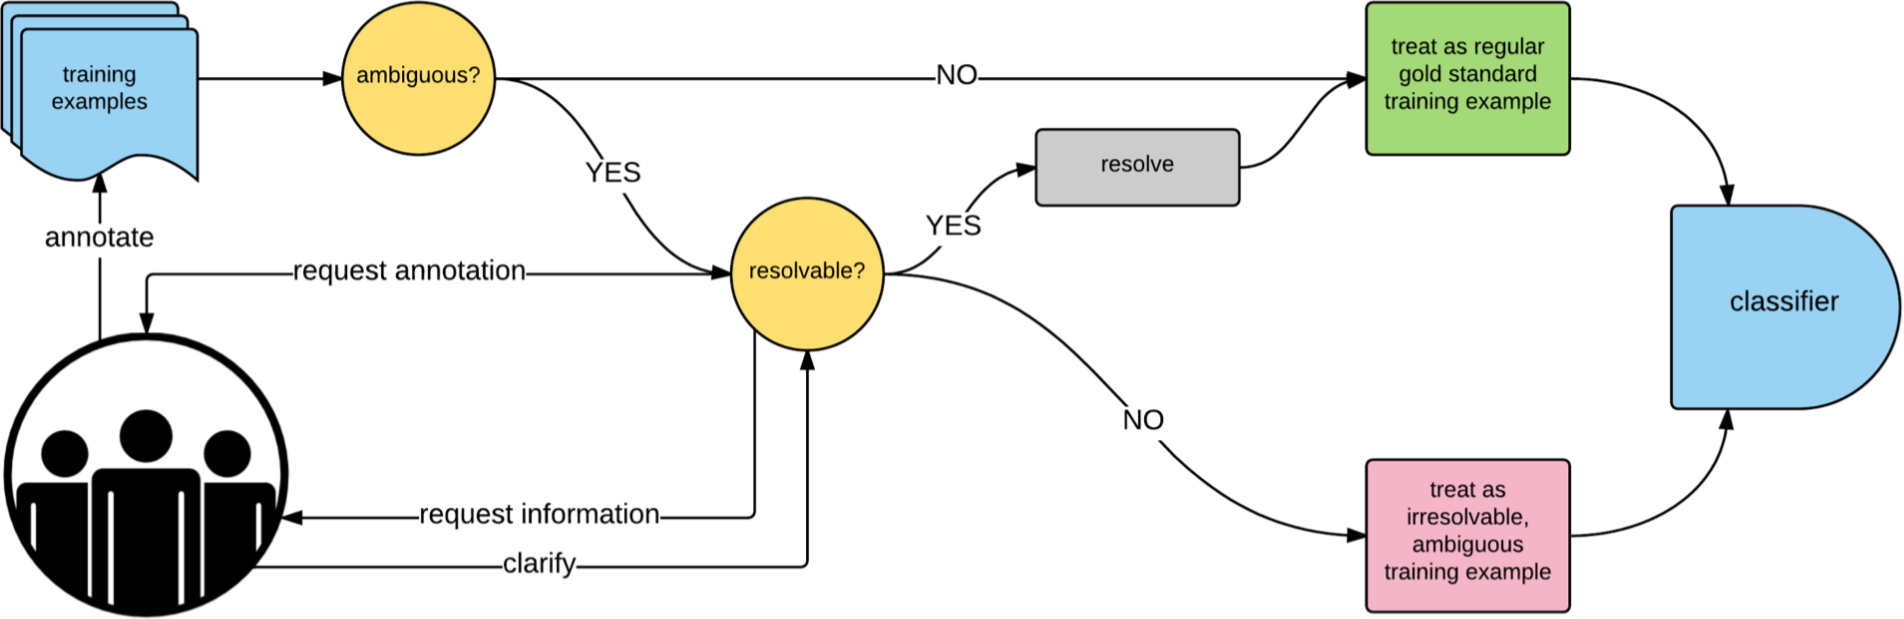
\includegraphics[width=14cm]{hcml-schematic}
\end{center}
\caption{A schematic diagram from \cite{schaekermann2016resolvable} for semi-automated transcription. This  framework is designed especially for resolving ambiguity, which is not the focus of my project. Nonetheless, this diagram depicts a collaborative framework betwee machine learning and human annotation.}
\label{fig:hcml-schematic}
\end{figure}

I refer to this as semi-automated transcription. This project presents a pipeline for semi-automated transcription, blending the irreplicable abilities of the human eye with the efficiency and scalability of character recognition algorithms.



%
% Motivation
%
\section{Contributions}
The methods used in this project borrow heavily from methods in the aforementioned research areas, including keyword and character spotting \cite{sharma2015adapting,frinken2012novel}, word recognition \cite{howe2009finding}, and handwriting recognition \cite{fischer2013fast,bluche2013feature}.

Nonetheless, this project makes two notable contributions to the area of handwritten text recognition, both concerned with the challenges of damaged words. First, a framework for semi-automated transcription is detailed and implemented, in which damaged words could be labeled by an expert and seamlessly integrated into an otherwise automated word spotting process. The second contribution is an approach for virtually restoring damaged or low-quality words into a representation that could be recognized automatically.


\subsection{An Interactive Approach to Word Spotting}
A semi-automated approach to word spotting utilizes user-provided labels of words in a given document. Essentially, a group of users generate a training set, which allows the system to recognize most occurrences of a given word in the training set. If a distorted occurrence of the word exists, the system will leave it unlabeled and leave the word image in the pool of images to be labeled by users.


\subsection{A Technique for Virtual Ink Restoration}
Several techniques .




%\section{Literature Review}
%\subsection{2009}
%\begin{itemize}
%\item Finding words in alphabet soup: Inference on freeform character recognition for historical scripts \cite{howe2009finding}.
%\end{itemize}
%
%\subsection{2012}
%\begin{itemize}
%\item A novel word spotting method based on recurrent neural networks \cite{frinken2012novel}.
%\item End-to-end text recognition with convolutional neural networks \cite{wang2012end}.
%\end{itemize}
%
%\subsection{2013}
%\begin{itemize}
%\item Handwritten word recognition using mlp based classifier: A holistic approach \cite{acharyya2013handwritten}.
%\item Feature extraction with convolutional neural networks for handwritten word recognition \cite{bluche2013feature}.
%\end{itemize}
%
%\subsection{2014}
%\begin{itemize}
%\item A combined system for text line extraction and handwriting recognition in historical documents \cite{fischer2014combined}
%\end{itemize}
%
%\subsection{2015}
%\begin{itemize}
%\item Efficient segmentation-free keyword spotting in historical document collections \cite{rusinol2015efficient}.
%\item Adapting off-the-shelf cnns for word spotting \& recognition \cite{sharma2015adapting}.
%\item Segmentation-free handwritten Chinese text recognition with LSTM-RNN \cite{messina2015segmentation}.
%\end{itemize}
%
%\subsection{2016}
%\begin{itemize}
%\item On the Benefits of Convolutional Neural Network Combinations in Offline Handwriting Recognition \cite{suryani2016benefits}.
%\item Reading text in the wild with convolutional neural networks \cite{jaderberg2016reading}.
%\item PHOCNet: A deep convolutional neural network for word spotting in handwritten documents \cite{sudholt2016phocnet}.
%\item SpottingNet: Learning the Similarity of Word Images with Convolutional Neural Network for Word Spotting in Handwritten Historical Documents \cite{zhong2016spottingnet}.
%\end{itemize}
%
%\subsection{Surveys}
%\begin{itemize}
%\item A survey of document image word spotting techniques \cite{giotis2017survey}.
%
%\item A survey on handwritten documents word spotting \cite{ahmed2017survey}.
%\end{itemize}





%%
%
%
% Methodology Chapter
%
%%
\chapter{Methodology}


%
% Motivation
%
\section{Preprocessing}
For the George Washington dataset, segmented and binarized word images are already provided. For the Wycliffe dataset, several preprocessing steps must be taken to get from raw images of the manuscript to segmented, binarized word images suitable for word spotting. 

\subsection{Alignment}

\begin{figure}[t]
\begin{center}
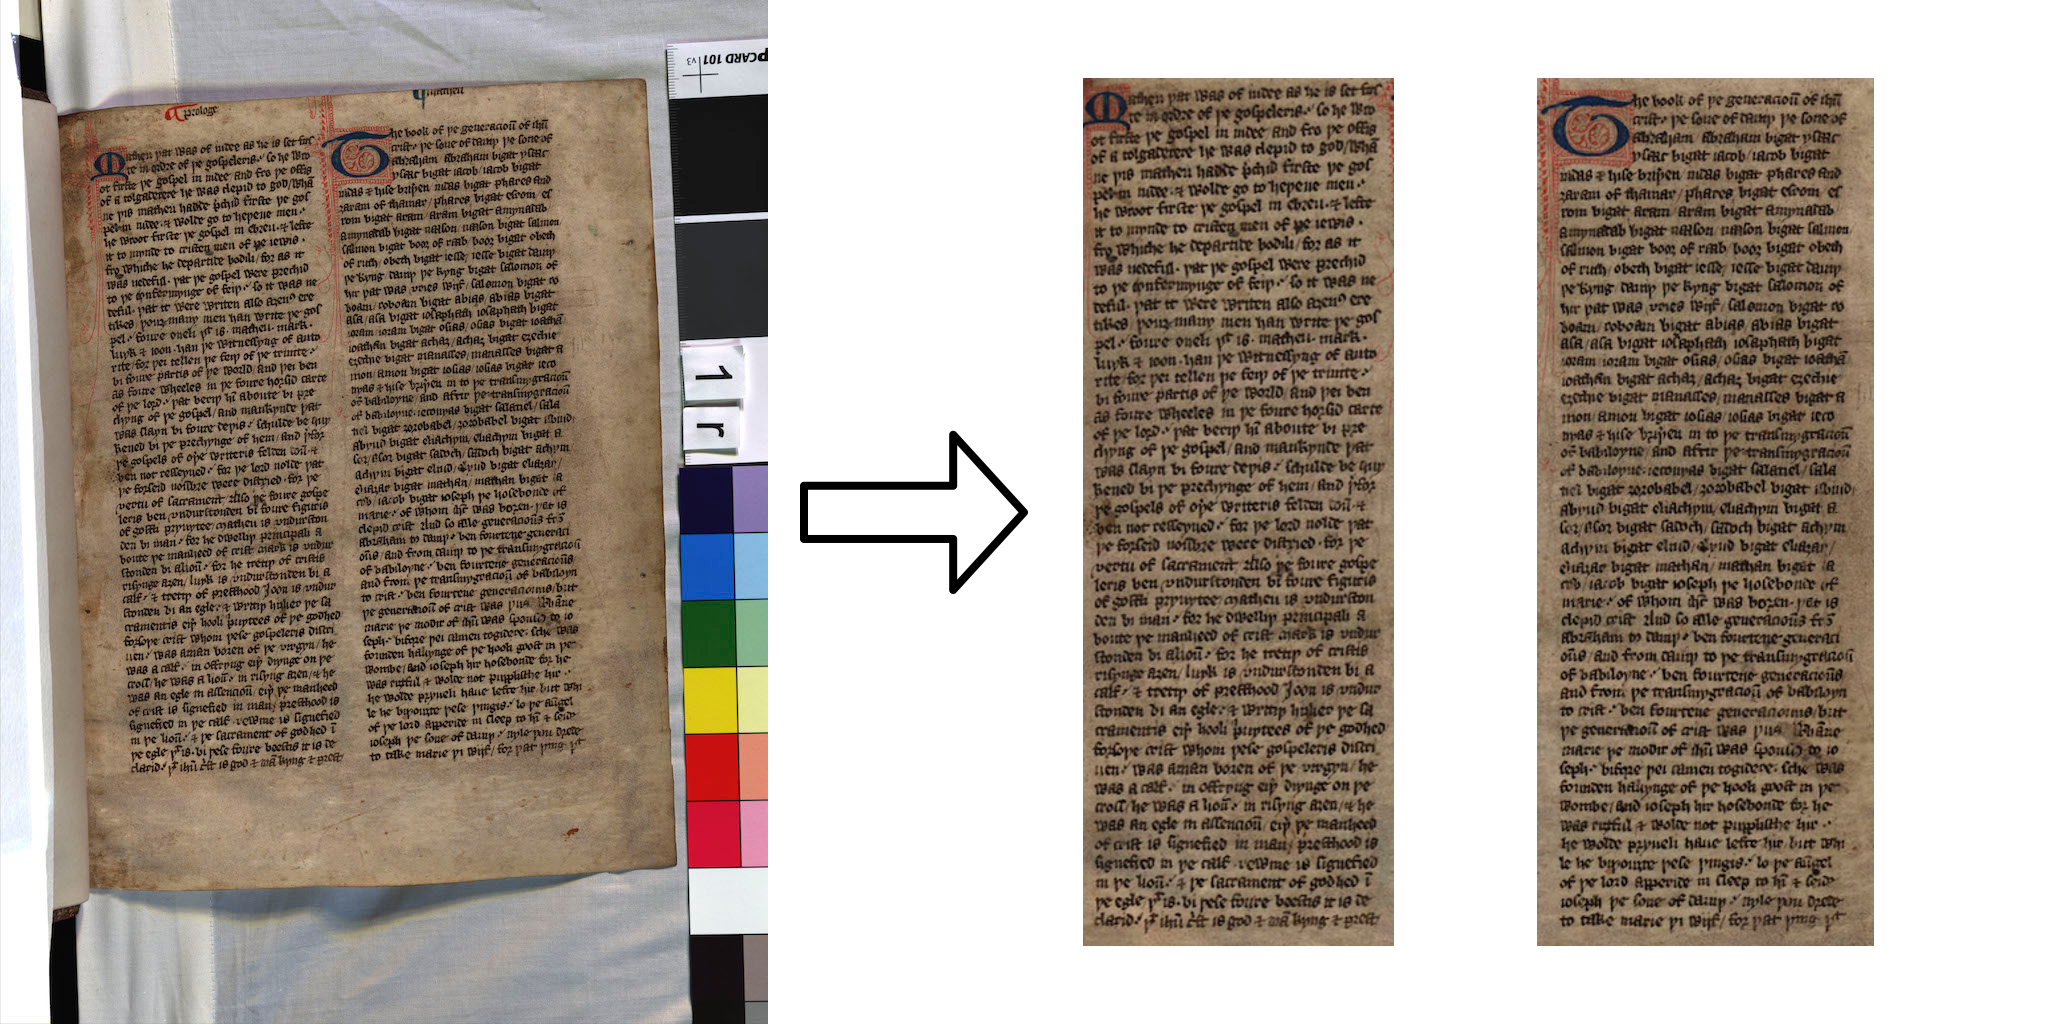
\includegraphics[width=14cm]{rotate-crop}
\end{center}
\caption{A sample of the original photographs of the Wycliffe New Testament Manuscript. In the preprocessing phase, these images must be aligned and cropped into separate columns.}
\label{fig:rotate-crop}
\end{figure}
The first step, visualized in figure \ref{fig:rotate-crop}, involves rotating the original photographs so that text columns are vertically aligned. Rotation varies depending on where the page existed in the binding and which side of the book it was on.

Columns were cropped identically on each page, based on the assumption that more precise segmentation would take place in the line segmentation and word segmentation algorithms. The key in column cropping is to create images that only contain text from one column. The amount of margin outside the column need not be precise, however, to allow for key assumptions in the binarization phase, it must not contain anything besides paper.


\subsection{Binarization}
Once the column images are cropped, the RGB image is flattened into a single grayscale channel. The image is then inverted so that the text is white and the background dark gray. To remove the gray background, the system uses a thresholding algorithm implemented by OpenCV \cite{bradski2000opencv}. Because lighting and coloring varies across manuscript pages, a global threshold would lead to noisy and inconsistent background removal. Instead, a threshold should be calculated individually for each page.

Because the column image is assumed to only contain ink and paper, a histogram of values in the column image should be bimodal (the two peaks representing the approximate value of an ink pixel and a paper pixel). Otsu's binarization algorithm \cite{otsu1979threshold} takes advantage of this bimodal distribution. It works by choosing a threshold value in between the two peaks that minimizes the variance within the two ``classes,'' an ideal method for these manuscript pages.


\subsection{Segmentation}
After column images are binarized, the next step is to split the column into its individual lines and words.

The Wycliffe New Testament is aligned and spaced with remarkable consistency. So, the segmentation involved plotting a vertical projection profile of a page image to determine the location of individual lines of text. To segment the line of text into individual words, in this case, a simple threshold on the horizontal projection profile provided sufficient accuracy. Because of the alignment, the intensity vector across the line had consistent valleys at the spaces in between each word.


\subsection{Damage Simulation}
The George Washington dataset, which is used for baseline testing, exists in fairly high quality.


\subsection{Feature Extraction}
Two methods were used for feature extraction. Histogram of oriented gradients (HOG) features were used as a baseline, and extracted using a scikit-image implementation \cite{van2014scikit}. The second method, the VAE's encoded representation of images, is detailed in the following section.



%
% VAE Details
%
\section{Variational Autoencoder}

The purpose of the VAE is to learn an encoded representation of the word images without the need for ground truth label. The general structure of a VAE trains by encoding its input then attempting to recreate it using the decoder. Backwards propagation of error occurs based on how similar the decoded image is to the original input image. Thus, a successful encoding allows the decoder to accurately recreate the input image. This process is visualized in figure \ref{fig:vaedemo}.

Figure blank shows. The experiment used two different architectures to determine the effect of expanding or contracting the size of the encoded layer, both were implemented using Keras \cite{chollet2015keras} with TensorFlow \cite{abadi2016tensorflow} used as the backend.


\section{Clustering}
To determine which word images contain the same word, clustering is performed on the encoded representation of the word images. The experiment tried two different clustering schemes: k-means and agglomerative. K-means is a popular centroid-based approach which iteratively refines the approximated center of each cluster \cite{lloyd1982least,likas2003global}. On the other hand, agglomerative clustering works by repeatedly merging the two closest clusters, resulting in a dendrogram with a single ``cluster" at one end and n ``clusters" at the other, where n is the number of data points.

Agglomerative clustering provides a natural fit for clustering encoded word images. Intuitively, each step groups the two most similar images into the same cluster. So instead of defining the number of clusters before the algorithm starts, the algorithm can stop when the two most similar images differ by a given amount.


\section{Priority Queue}
In the current approach, images are labeled in the order which they appear. However, this can be modified depending on the need of the given task. For example, if a general understanding of the document's contents is more important than a word-for-word transcription, the system could request labels for frequently occurring words. Or, for partially damaged documents, the system could request labels for ``misfit" words that are particularly confusing to the encoder or to the clustering algorithm.


\section{Providing Labels}
Labels are provided in a simple graphical user interface which displays the original word image (before inverting it and removing the background). The interface, built using TKInter, allows a user to type in a label for the word image, skip to the next word, or flag the word image as needing re-segmentation.

In the experiments, a simulated oracle was used for labeling. Because the word images were sorted in order of appearance in the text, the oracle simply labeled the image using the word at the corresponding index of the transcript.


\section{Transcription}
A transcription of the full set of word images can be given at any time. Each word image must be encoded by the network. The encoded representation is used to determine which cluster of images the word belongs to. Once a word image is clustered, transcribing it is simply a matter of applying the label for that cluster. If the cluster is unlabeled, words in that cluster will show up in the transcript as ``unknown." 




%%
%
%
% Evaluation Chapter
%
%%
\chapter{Evaluation}
There were two goals in the evaluation phase. First, to determine whether the VAE's encoded representation of images could be used as features in the clustering phase of word spotting. The second goal was to determine whether the VAE could reconstruct damaged words so as to accurately classify them during word spotting.


%
% Data Background Section
%
\section{Data Background}
Two datasets were used to evaluate the interactive approach to word recognition and ink restoration.

\subsection{George Washington Dataset}
The George Washington Dataset is enormously popular for evaluating handwriting recognition.

The subset of data used in this paper is from work done by \cite{fischer2012lexicon}. The authors provide word segmentation, ground truth, and normalized images for 20 pages of the George Washington letters.

\subsection{Wycliffe Dataset}


%
% George Washington Results
%
\section{Classification on George Washington Dataset}
Results from experiments on original word images.

\begin{center}
\includegraphics[width=10cm]{results-placeholder}
\end{center}



%
% George Washington Results
%
\section{Classification on ``Damaged'' George Washington Dataset}
Results from experiments on damaged words.

\begin{center}
\includegraphics[width=10cm]{results-placeholder}
\end{center}


%
% Wycliffe Data Results
%
\section{Wycliffe New Testament}
Results from experiments on the Wycliffe dataset. First four pages or so?

\begin{center}
\includegraphics[width=10cm]{results-placeholder}
\end{center}





%%
%
%
% Introduction Chapter
%
%%
\chapter{Conclusion}

\section{Challenges}
What I ran into.

\section{Findings}
What I found.

\section{Future Work}
Suggestions for future work.





%%
%
%
% Evaluation Chapter
%
%%
\chapter{The Example Chapter}
\section{The Example Section}
Math goes here.
\begin{figure}[h]
\centering
Here's a figure
\caption{A Simple Figure}
\end{figure}
\begin{table}[h]
\centering
\begin{tabular}{c|c}
Here & is \\
\hline
a & table
\end{tabular}
\caption{A Simple Table}
\end{table}
\copyrightnotice
%-----------------------------------------------
\backmatter
\bibliographystyle{unsrt}   % this means that the order of references
			    % is dtermined by the order in which the
			    % \cite and \nocite commands appear
\bibliography{mybib}  % list here all the bibliographies that
			     % you need. 

\chapter{Vita}
A brief vita goes here.
\end{document}